% Moved from the main text during the length revision. Content unchanged.
\begin{figure}[t]
\centering
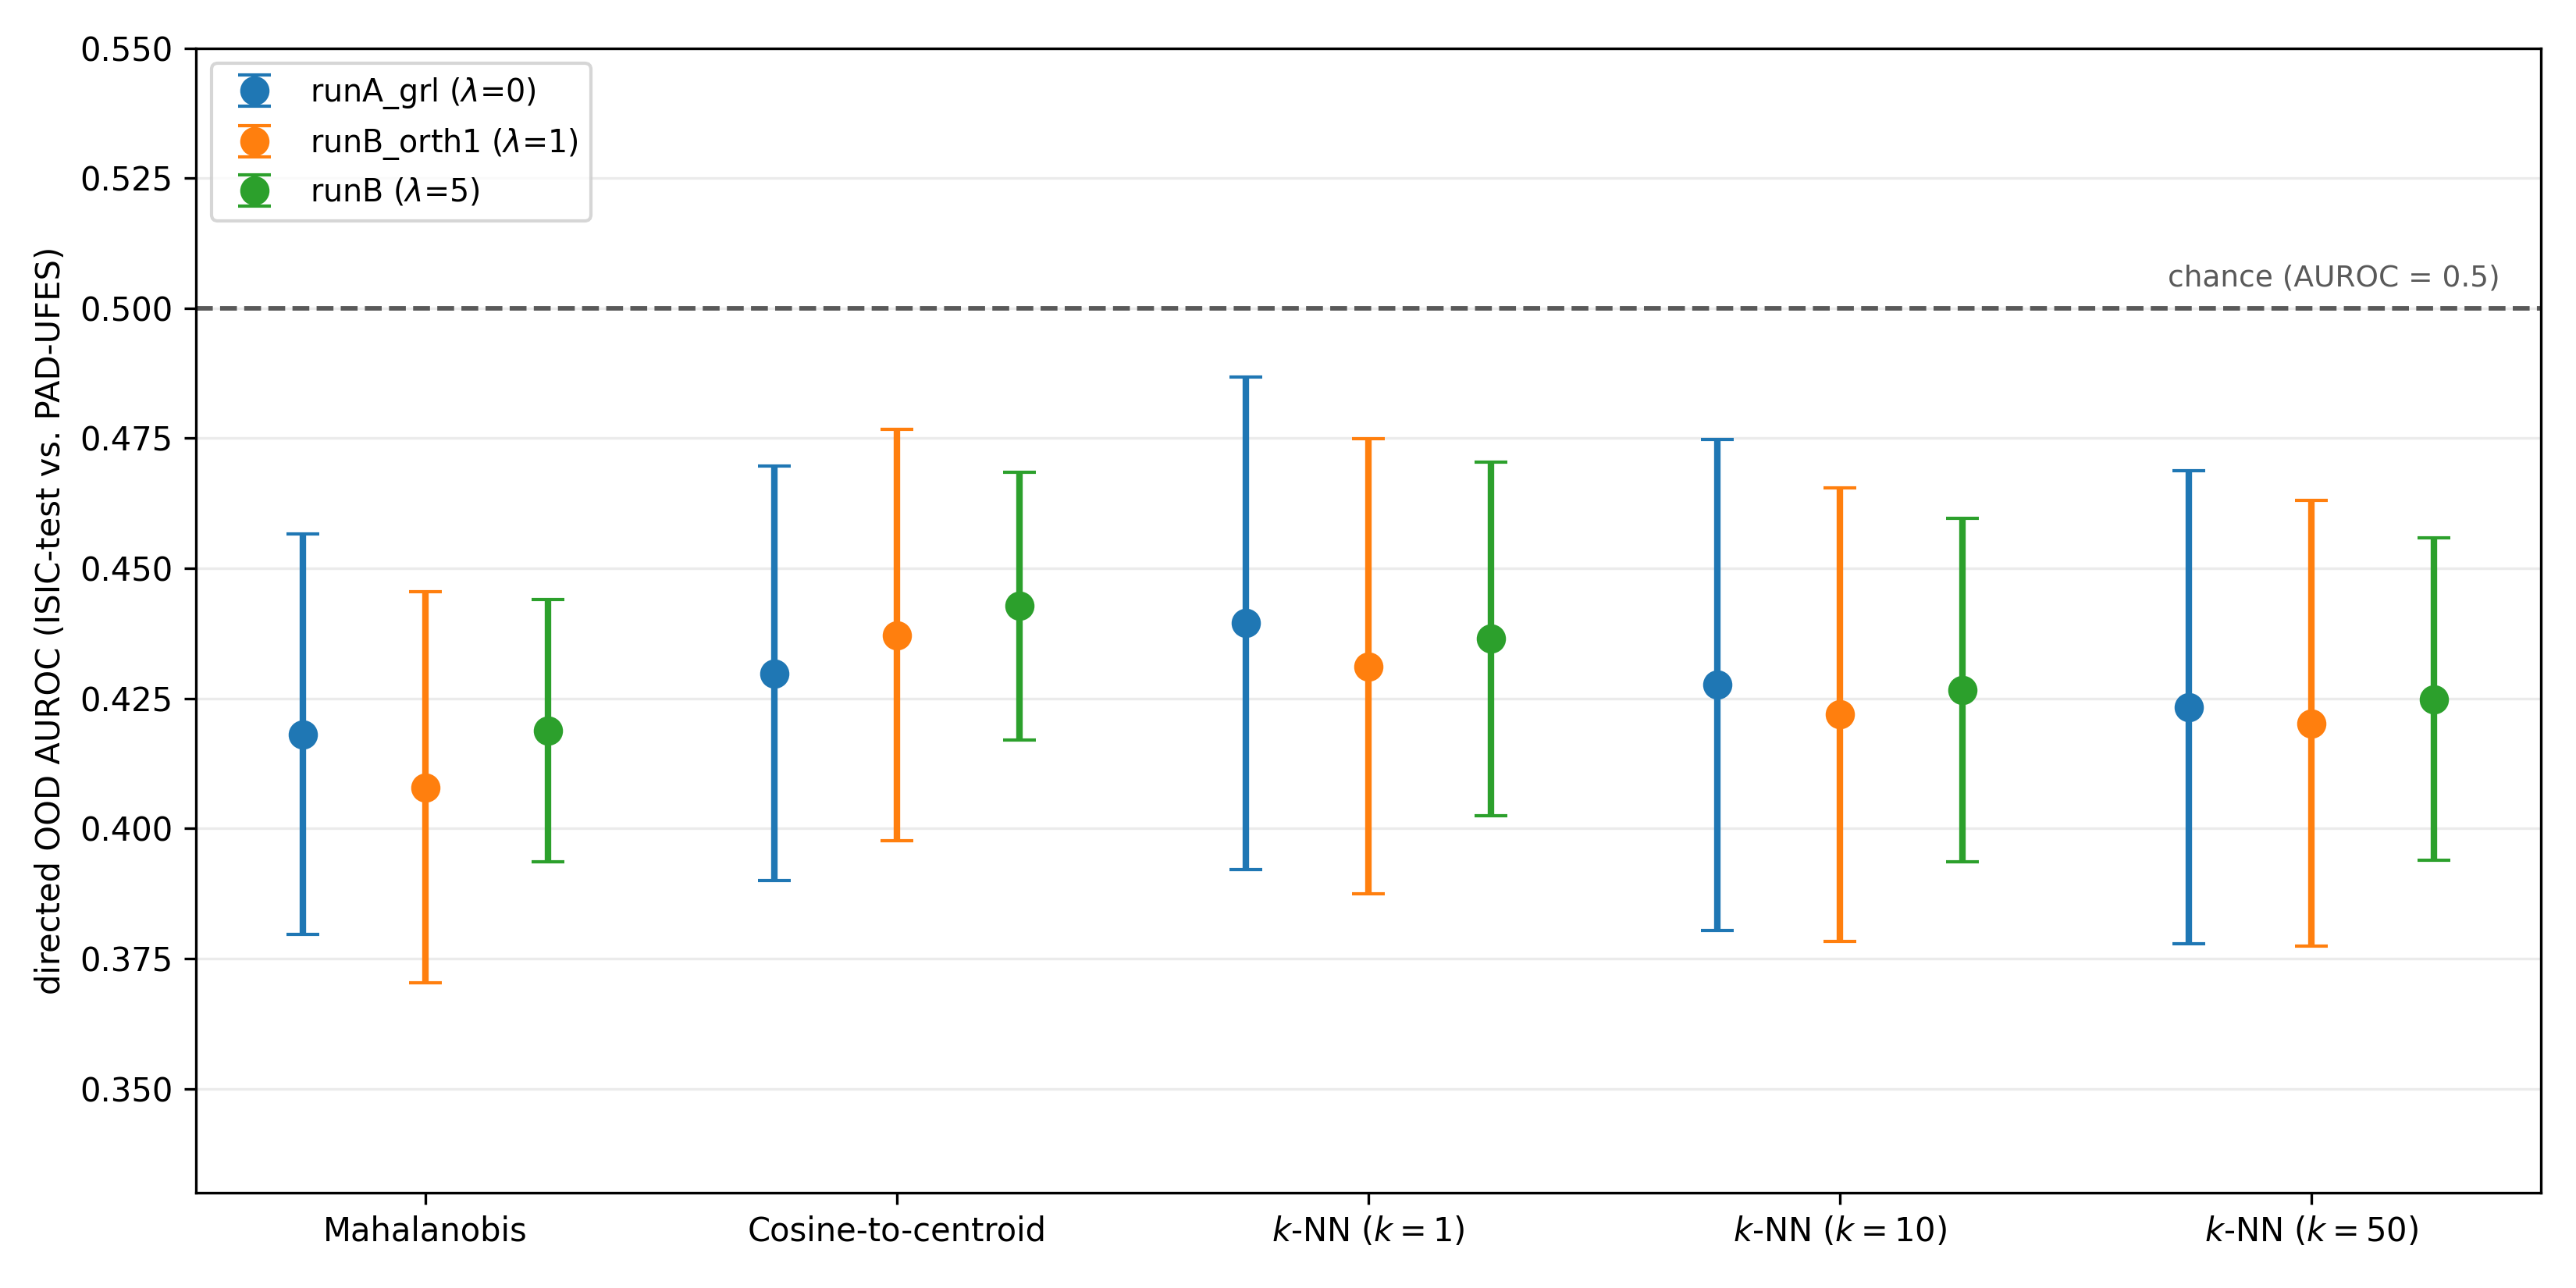
\includegraphics[width=0.6\linewidth]{figs/fig5_three_scorers.png}
\caption{Three distance-based scorer families are directionally misaligned alike. Directed OOD AUROC (ISIC-test vs.\ PAD-UFES) for Mahalanobis distance, cosine-to-centroid similarity, and pooled $k$-nearest-neighbor distance ($k = 1, 10, 50$), computed on the identical embeddings and grouped by rung (mean $\pm$ SD across seeds). Dashed line: chance (AUROC $= 0.5$). All five variants fall within 0.40--0.42 under the pre-specified higher-distance-is-more-OOD convention; their pooled orientation-free separability is 0.576--0.598 (Table~\ref{tab:five-scorers}, Panel B).}
\label{fig:five-scorers}
\end{figure}
